% Graphic for TeX using PGF
% Title: C:\Documents and Settings\Admin\Мои документы\Мои рисунки\Диаграмма1.dia
% Creator: Dia v0.97.2
% CreationDate: Sat Sep 08 10:36:26 2012
% For: Admin
% \usepackage{tikz}
% The following commands are not supported in PSTricks at present
% We define them conditionally, so when they are implemented,
% this pgf file will use them.
\ifx\du\undefined
  \newlength{\du}
\fi
\setlength{\du}{15\unitlength}
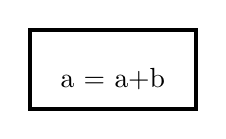
\begin{tikzpicture}
\pgftransformxscale{1.000000}
\pgftransformyscale{-1.000000}
\definecolor{dialinecolor}{rgb}{0.000000, 0.000000, 0.000000}
\pgfsetstrokecolor{dialinecolor}
\definecolor{dialinecolor}{rgb}{1.000000, 1.000000, 1.000000}
\pgfsetfillcolor{dialinecolor}
\definecolor{dialinecolor}{rgb}{1.000000, 1.000000, 1.000000}
\pgfsetfillcolor{dialinecolor}
\fill (5.050000\du,0.450000\du)--(5.050000\du,2.350000\du)--(9.050000\du,2.350000\du)--(9.050000\du,0.450000\du)--cycle;
\pgfsetlinewidth{0.100000\du}
\pgfsetdash{}{0pt}
\pgfsetdash{}{0pt}
\pgfsetmiterjoin
\definecolor{dialinecolor}{rgb}{0.000000, 0.000000, 0.000000}
\pgfsetstrokecolor{dialinecolor}
\draw (5.050000\du,0.450000\du)--(5.050000\du,2.350000\du)--(9.050000\du,2.350000\du)--(9.050000\du,0.450000\du)--cycle;
% setfont left to latex
\definecolor{dialinecolor}{rgb}{0.000000, 0.000000, 0.000000}
\pgfsetstrokecolor{dialinecolor}
\node at (7.050000\du,1.640000\du){a = a+b};
\end{tikzpicture}
